\documentclass[11pt, twocolumn]{article}
\usepackage{titlesec}
\usepackage{tikz}
\usepackage{booktabs}
\usepackage{adjustbox} 
\usepackage{enumitem}
\usepackage{multirow}
\usepackage{bbding,enumitem}
\usepackage{authblk}
\usepackage{fancyhdr}
\usepackage{amsmath}
\usepackage{subcaption}
\usepackage[table]{xcolor}
\setcounter{secnumdepth}{3} % for adjusting padding
\pagestyle{fancy}
\newcommand{\blueoval}{%
    \begin{tikzpicture}[remember picture, overlay]
    \shade[shading=axis, left color=blue, right color=white] (current page.north west) -- (3,0) arc (0:180:4cm) -- cycle;
    \end{tikzpicture}%
}

\newcommand{\coloredfooter}{%
    \begin{tikzpicture}[remember picture, overlay]
    \shade[shading=axis, left color=teal, right color=white] (current page.south east) -- (-1,-2) arc (0:80:2cm) -- cycle;
    \end{tikzpicture}%
}

\fancyhf{} % Clear default header and footer
\fancyhead[L]{ \leftmark}
% Display section title in the left header
\fancyhead[R]{\thepage} % Display page number in the right header
\definecolor{mypink3}{cmyk}{0, 0.7808, 0.4429, 0.1412}

\makeatletter
\renewcommand{\maketitle}{\bgroup\setlength{\parindent}{0pt}
\begin{flushleft}
  \textbf{\@title}

  \@author
\end{flushleft}\egroup
}
\makeatother

\title{\Huge \color{mypink3}{ROV Document}  \vspace{0.5cm}}
\author{\Large E-JUST Robotics Club \normalsize \hspace{0.5cm} }

\setlength{\parindent}{0pt}
\date{\today}

\usepackage[showframe=false, margin=.75in]{geometry}

\usepackage{abstract}
\renewcommand{\abstractname}{}    % clear the title
\renewcommand{\absnamepos}{empty} % originally center

\usepackage{lipsum}

\usepackage{afterpage}

\renewenvironment{abstract}
 {\small
  \begin{center}
  \bfseries \abstractname\vspace{-.5em}\vspace{0pt}
  \end{center}
  \list{}{%
    \setlength{\leftmargin}{10mm}% <---------- Change margin here
    \setlength{\rightmargin}{\leftmargin}%
  }%
  \item\relax}
 {\endlist}

\usepackage[utf8]{inputenc}

%\usepackage{graphicx}
\usepackage{wrapfig}
\usepackage[lofdepth,lotdepth]{subfig}
\usepackage{booktabs}

\usepackage{rotating}

\usepackage{caption}
%\usepackage{subcaption}

%\usepackage[ngerman]{babel}

\usepackage{csquotes}

\setlength{\marginparwidth}{2cm} % Set marginparwidth to avoid todonotes issues
\usepackage{todonotes}

\usepackage{stfloats}

\usepackage[T1]{fontenc}
\usepackage{textcomp}
\usepackage{times}

\usepackage{framed} %um Boxen zu machen

\usepackage[citestyle=authoryear,
			bibstyle=authoryear,
			language=auto,
			url=false,
			backend=bibtex,
			doi=false,
			isbn=false]{biblatex}
	\renewbibmacro*{volume+number+eid}{%
  \printfield{volume}%
%  \setunit*{\adddot}% DELETED
  \setunit*{\addnbspace}% NEW (optional); there's also \addnbthinspace
  \printfield{number}%
  \setunit{\addcomma\space}%
  \printfield{eid}}
\DeclareFieldFormat[article]{number}{\mkbibparens{#1}}

\usepackage{setspace}
\onehalfspacing

\setlength{\columnsep}{0.8cm}

\setlength{\parskip}{0em}

\usepackage{color}
\definecolor{black}{gray}{0} % 10% gray

\usepackage[colorlinks=true,linkcolor=black,citecolor=black]{hyperref}

\usepackage{tabularx}
\newcolumntype{s}{>{\hsize=.5\hsize}X}

\usepackage{ntheorem}
\newtheorem*{TRQ}{Research Question}

\newtheorem{Hyp}{Hypothesis} 

\usepackage{graphicx}
\usepackage{fancyhdr}
\usepackage{lipsum}
\usepackage{geometry}
\usepackage{changepage} % To adjust page margins locally
\usepackage{afterpage}

% Apply the custom header and footer to all pages
\fancyfoot[L]{\hspace*{-1.9cm}{
\includegraphics[width=\paperwidth,height=1.9cm]{Images/Footer.png}}} % Footer

\pagestyle{fancy}
\makeatletter
\providecommand{\sf@counterlist}{} % Define sf@counterlist to avoid undefined control sequence
\makeatother

\usepackage{titlesec}

\titlespacing*{\subsection}{0pt}{5pt}{5pt}
\titlespacing*{\subsubsection}{0pt}{5pt}{5pt}

\setcounter{secnumdepth}{4}
\renewcommand\theparagraph{\thesubsubsection.\arabic{paragraph}}

\usepackage{tabularray}
\DefTblrTemplate{firsthead,middlehead,lasthead}{default}{}
\DefTblrTemplate{firstfoot}{default}{
  \UseTblrTemplate{contfoot}{default}
  \UseTblrTemplate{caption}{default}
}
\DefTblrTemplate{middlefoot}{default}{
  \UseTblrTemplate{contfoot}{default}
  \UseTblrTemplate{capcont}{default}
}
\DefTblrTemplate{lastfoot}{default}{
  \UseTblrTemplate{note}{default}
  \UseTblrTemplate{remark}{default}
  \UseTblrTemplate{capcont}{default}
}
\DefTblrTemplate{contfoot-text}{default}{Continue on the next column}
\DefTblrTemplate{capcont}{default}{\UseTblrTemplate{caption}{default}}
\UseTblrLibrary{booktabs}
\captionsetup{skip=3pt}
\SetTblrInner{rowsep=0pt, stretch=0.9}
\setlength{\headheight}{13.6pt}
\addtolength{\topmargin}{-1.6pt}
\setlength{\footskip}{58.2pt}

\begin{document}
\onecolumn

\tableofcontents
\clearpage

\section{Community Engagement}
At E-JUST Robotics Club, community engagement is at the heart of our mission. We actively mentor future innovators, organize events, and collaborate with other organizations to promote STEM education and sustainability awareness.

\subsection{Roboverse 3 – May 24, 2024, at E-JUST Headquarters}
\href{https://fb.me/e/3yvYdIh8P/}{Event Link}

\subsubsection{Attendees}
\begin{itemize}
    \item 800+ students from Egypt-Japan University of Science and Technology (E-JUST)
    \item 100+ students from different universities (including Alexandria University and Borg Al Arab Technological University) and high school students from Borg El Arab
\end{itemize}

At Roboverse 3, our club engaged with more than 900 students and educators, showcasing our ROV and emphasizing our commitment to STEM education and environmental sustainability. We provided attendees with opportunities to interact with our projects firsthand through various activities.

\subsubsection{ROV Showcase and Information Sharing}
\begin{itemize}
    \item We set up an interactive booth where attendees could observe our ROV in action and learn about its technical specifications and capabilities.
    \item Our team explained the journey of the competition,tition, our objectives, and how our participation contributes to STEM education.
    \item The audience had the opportunity to learn about the mission, tasks and how the ROV was developed for competition.
    \item Visitors engaged directly with ROV team members, exchanging insights on their experiences while collaboratively exploring enhancements for future competitions based on attendee feedback and suggestions.
\end{itemize}
\begin{figure}[h]
    \centering
    \begin{minipage}{0.48\textwidth}
        \centering
        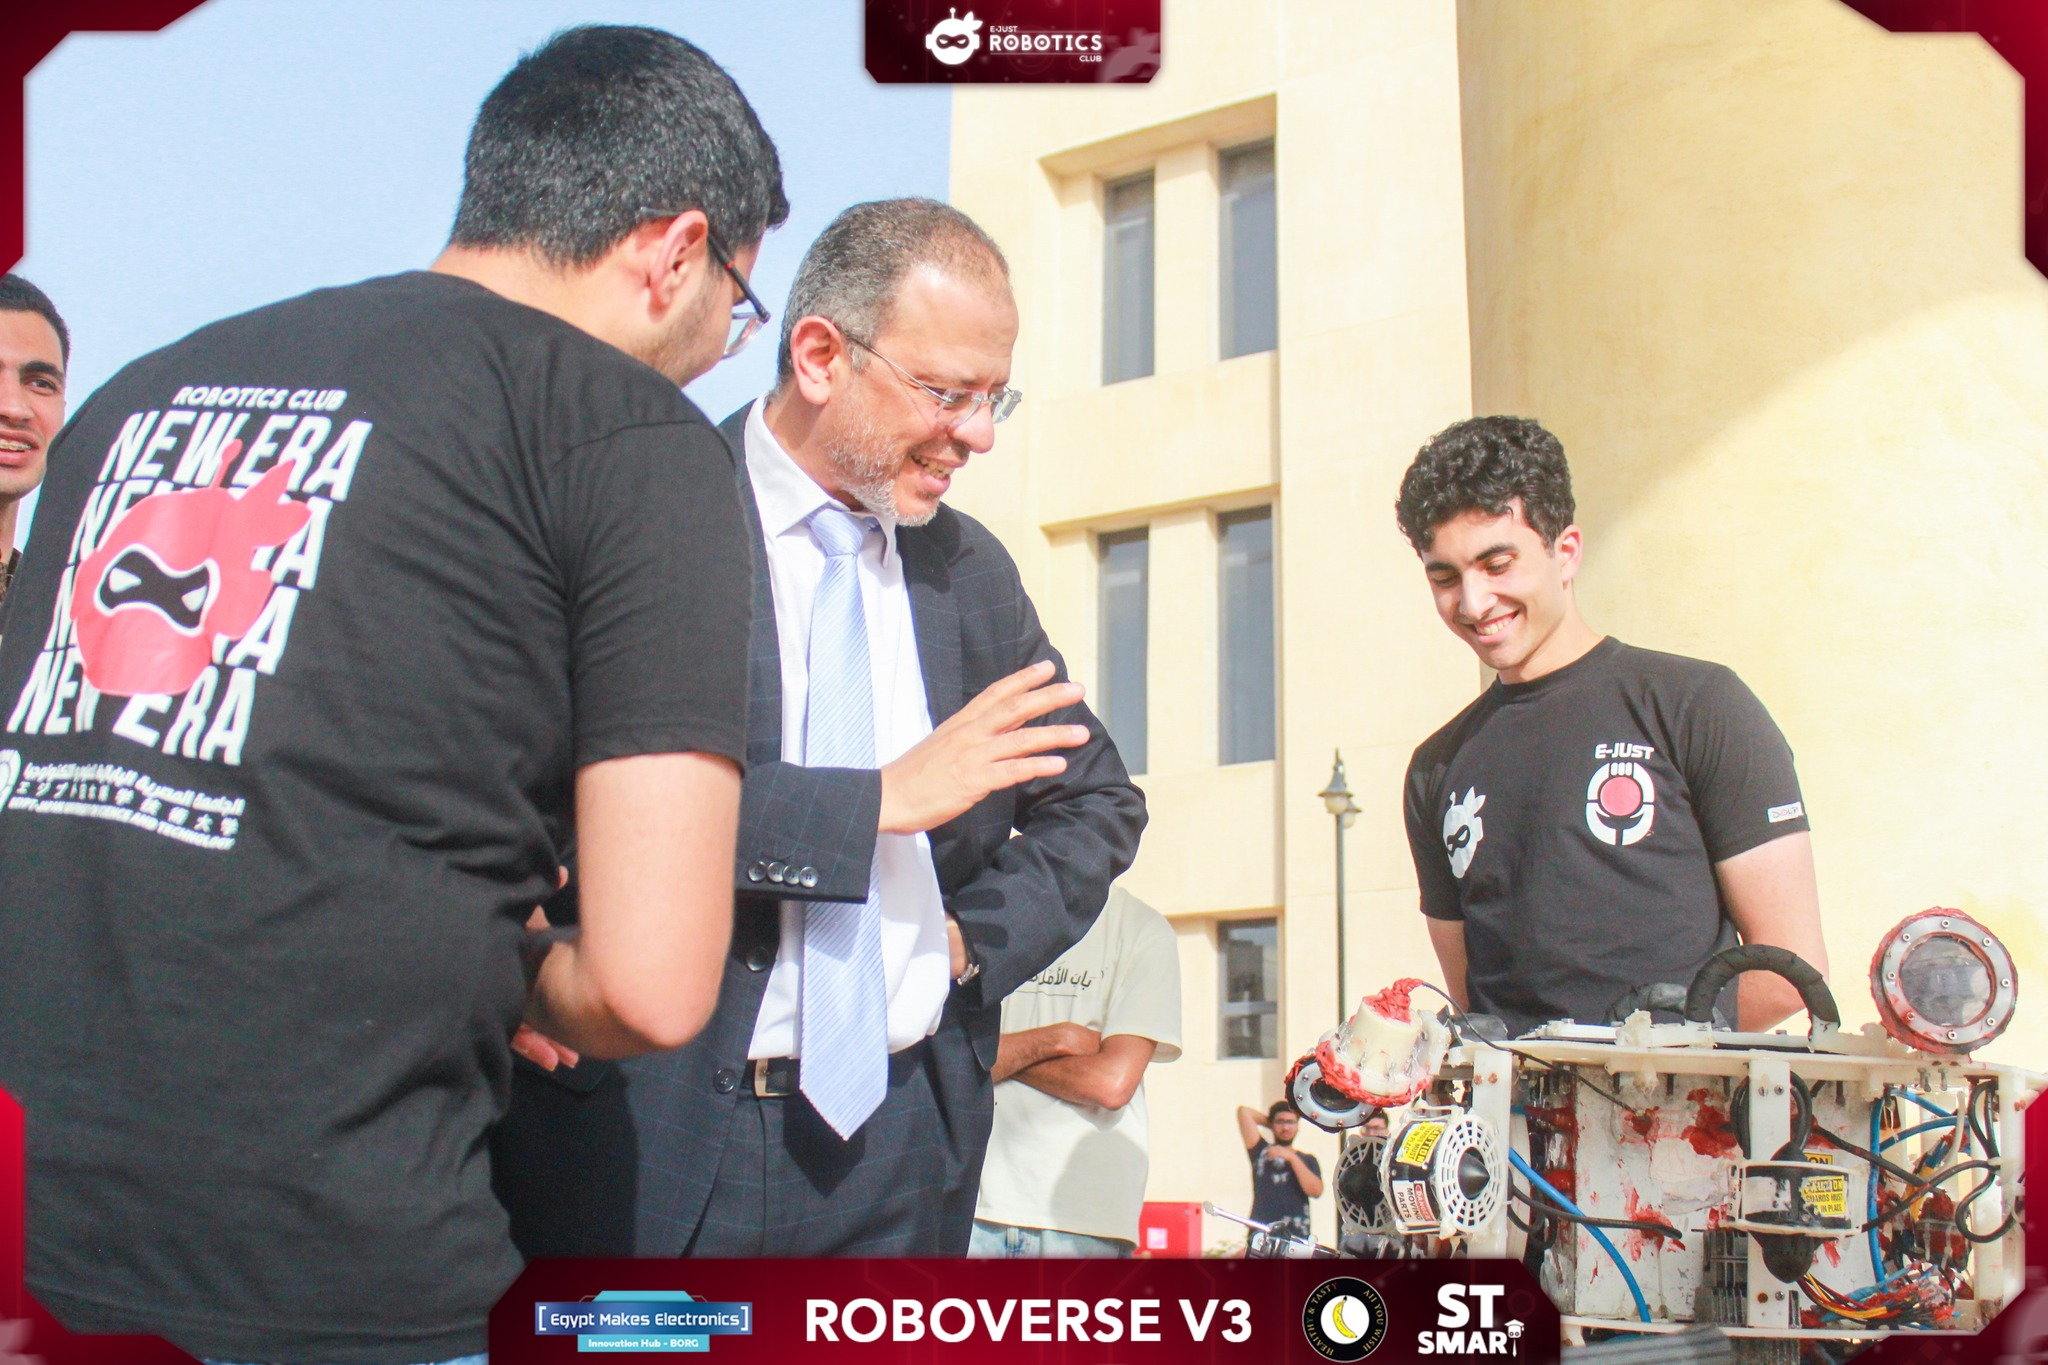
\includegraphics[width=\textwidth]{Images/ROV1.jpg}
        
        \label{fig:ROV1}
    \end{minipage}
    \hfill
    \begin{minipage}{0.48\textwidth}
        \centering
        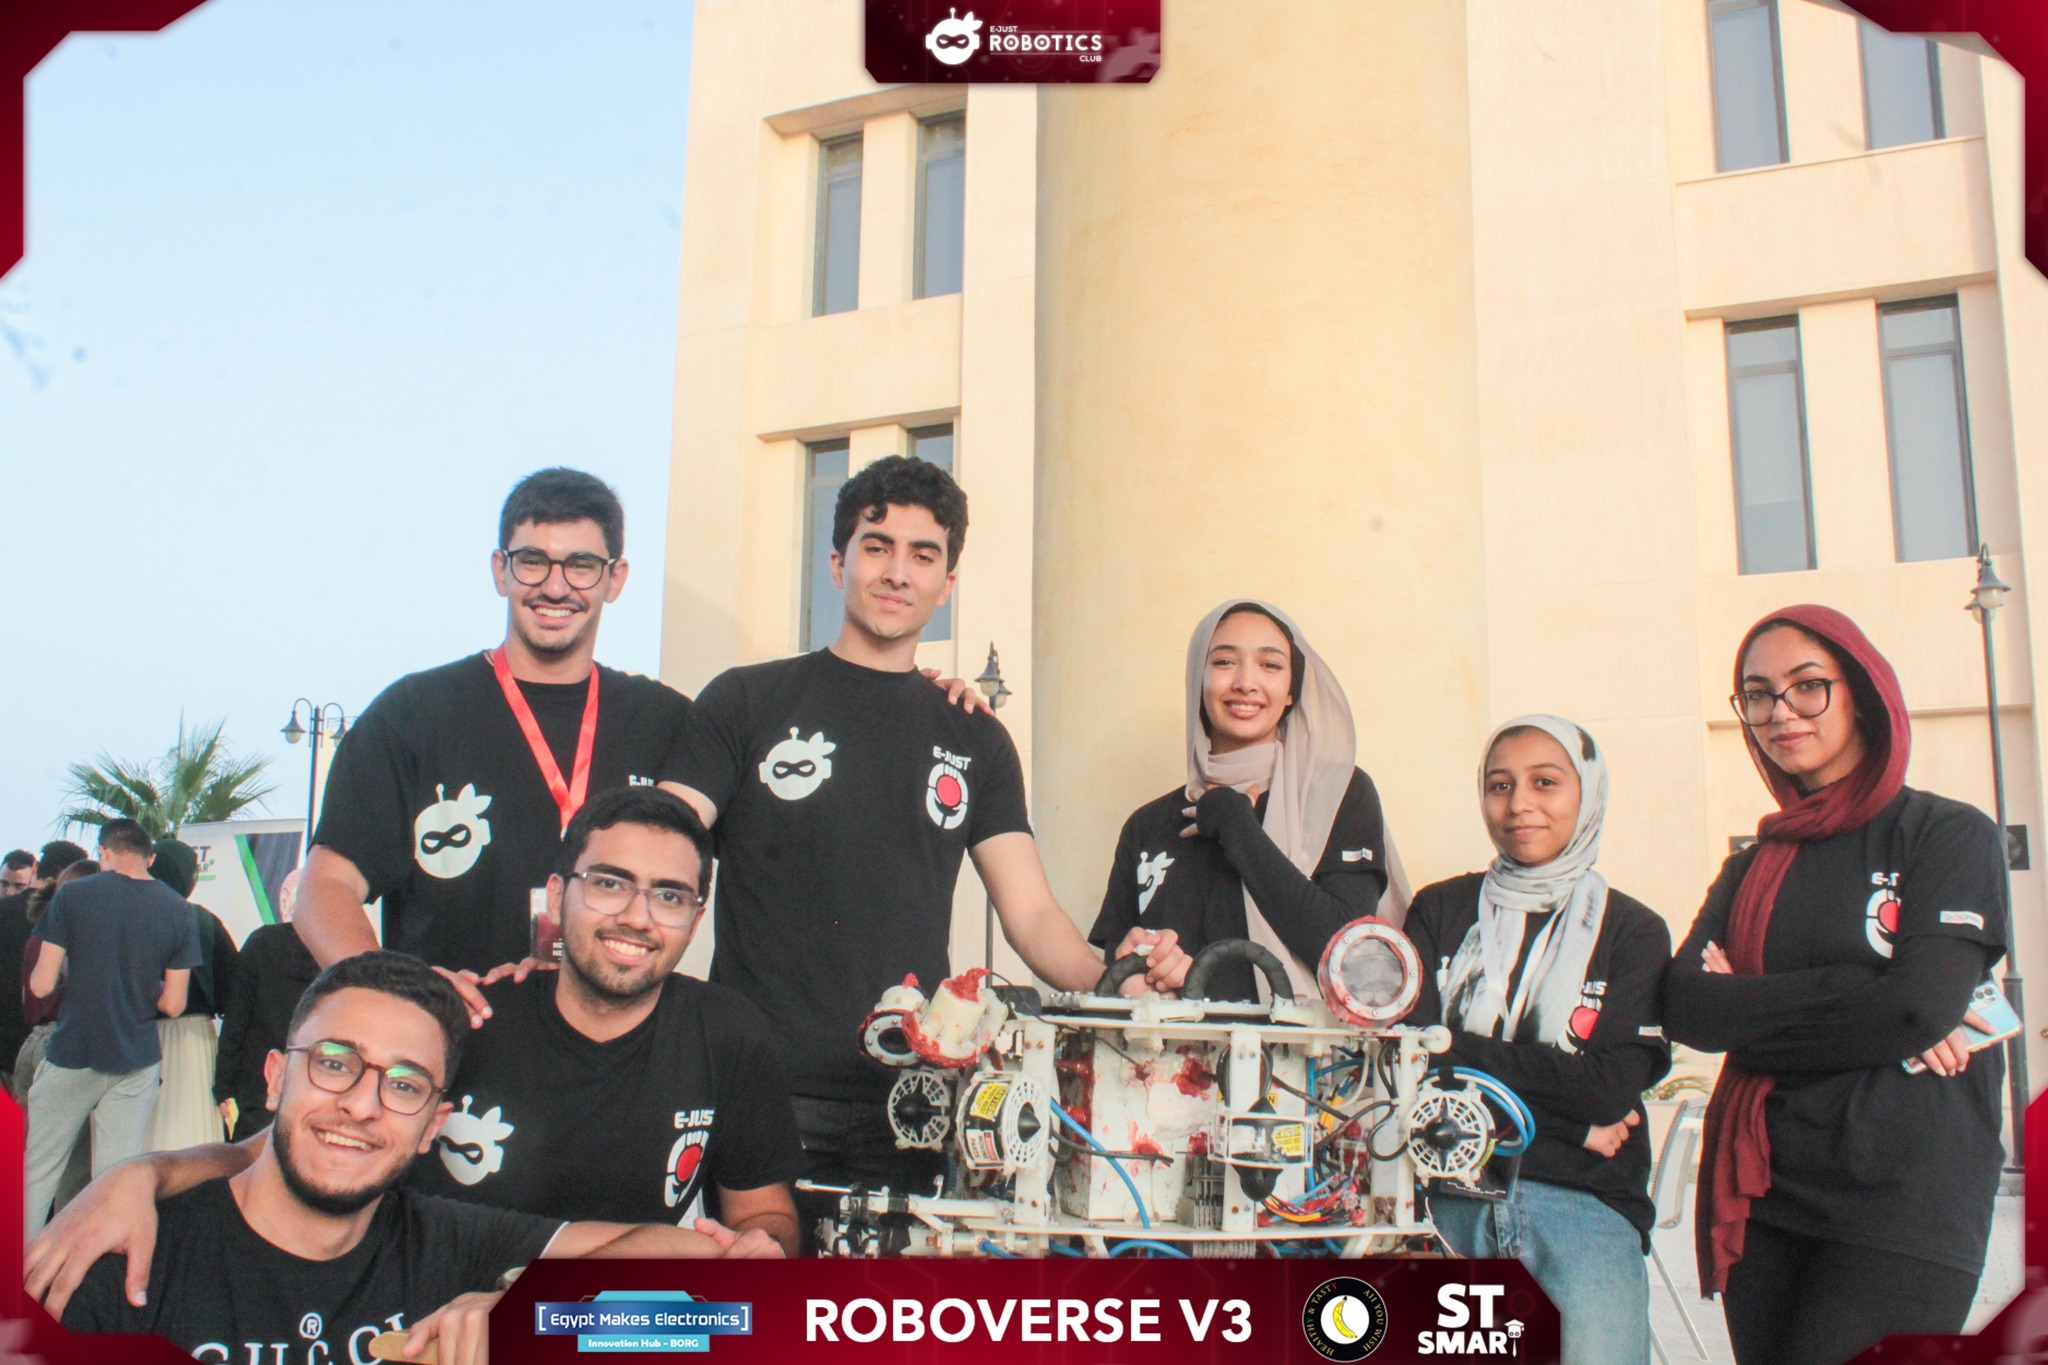
\includegraphics[width=\textwidth]{Images/ROV2.jpg}
      
        \label{fig:ROV2}
    \end{minipage}
    \caption{E-JUST Robotics Club ROV Team with Prof. Amr Eltawil, Dean of IDE School}
    \label{fig:ROV}
\end{figure}

\subsubsection{Q\&A Session and Technical Demonstrations}
\begin{itemize}
    \item We conducted detailed Q\&A sessions covering the technical aspects of our ROV and the challenges of underwater robotics.
    \item Participants engaged in in-depth discussions about our mission, design innovations, and the role of robotics in marine exploration.
\end{itemize}

\subsubsection{Showcasing Other Projects}
\begin{itemize}
    \item Attendees had hands-on experiences with interactive projects such as the Object Sorting Project, allowing them to explore robotics in action.
    \item Various club-developed projects were demonstrated, highlighting their real-world applications and engaging participants in workshops and activities.
\end{itemize}

\subsubsection{Collaboration with E-JUST Environmental Club}
\begin{itemize}
    \item We partnered with the E-JUST Environmental Club to promote sustainability and environmental responsibility.
    \item Activities included a planting workshop and discussions on Environmental, Social, and Governance (ESG) principles.
\end{itemize}

\subsubsection{Entertainment}
\begin{itemize}
    \item To enhance engagement, we introduced a variety of interactive games developed by our club members, including virtual bowling and a customized version of Subway Surfers.
    \item Attendees also enjoyed giveaways, a photobooth for capturing memorable moments, and competitive games that added excitement and fostered team spirit.
    \item These elements enriched the overall experience, seamlessly blending education with entertainment to create an engaging and dynamic event.
\end{itemize}
\begin{figure}[h]
    \centering
    \begin{minipage}{0.48\textwidth}
        \centering
        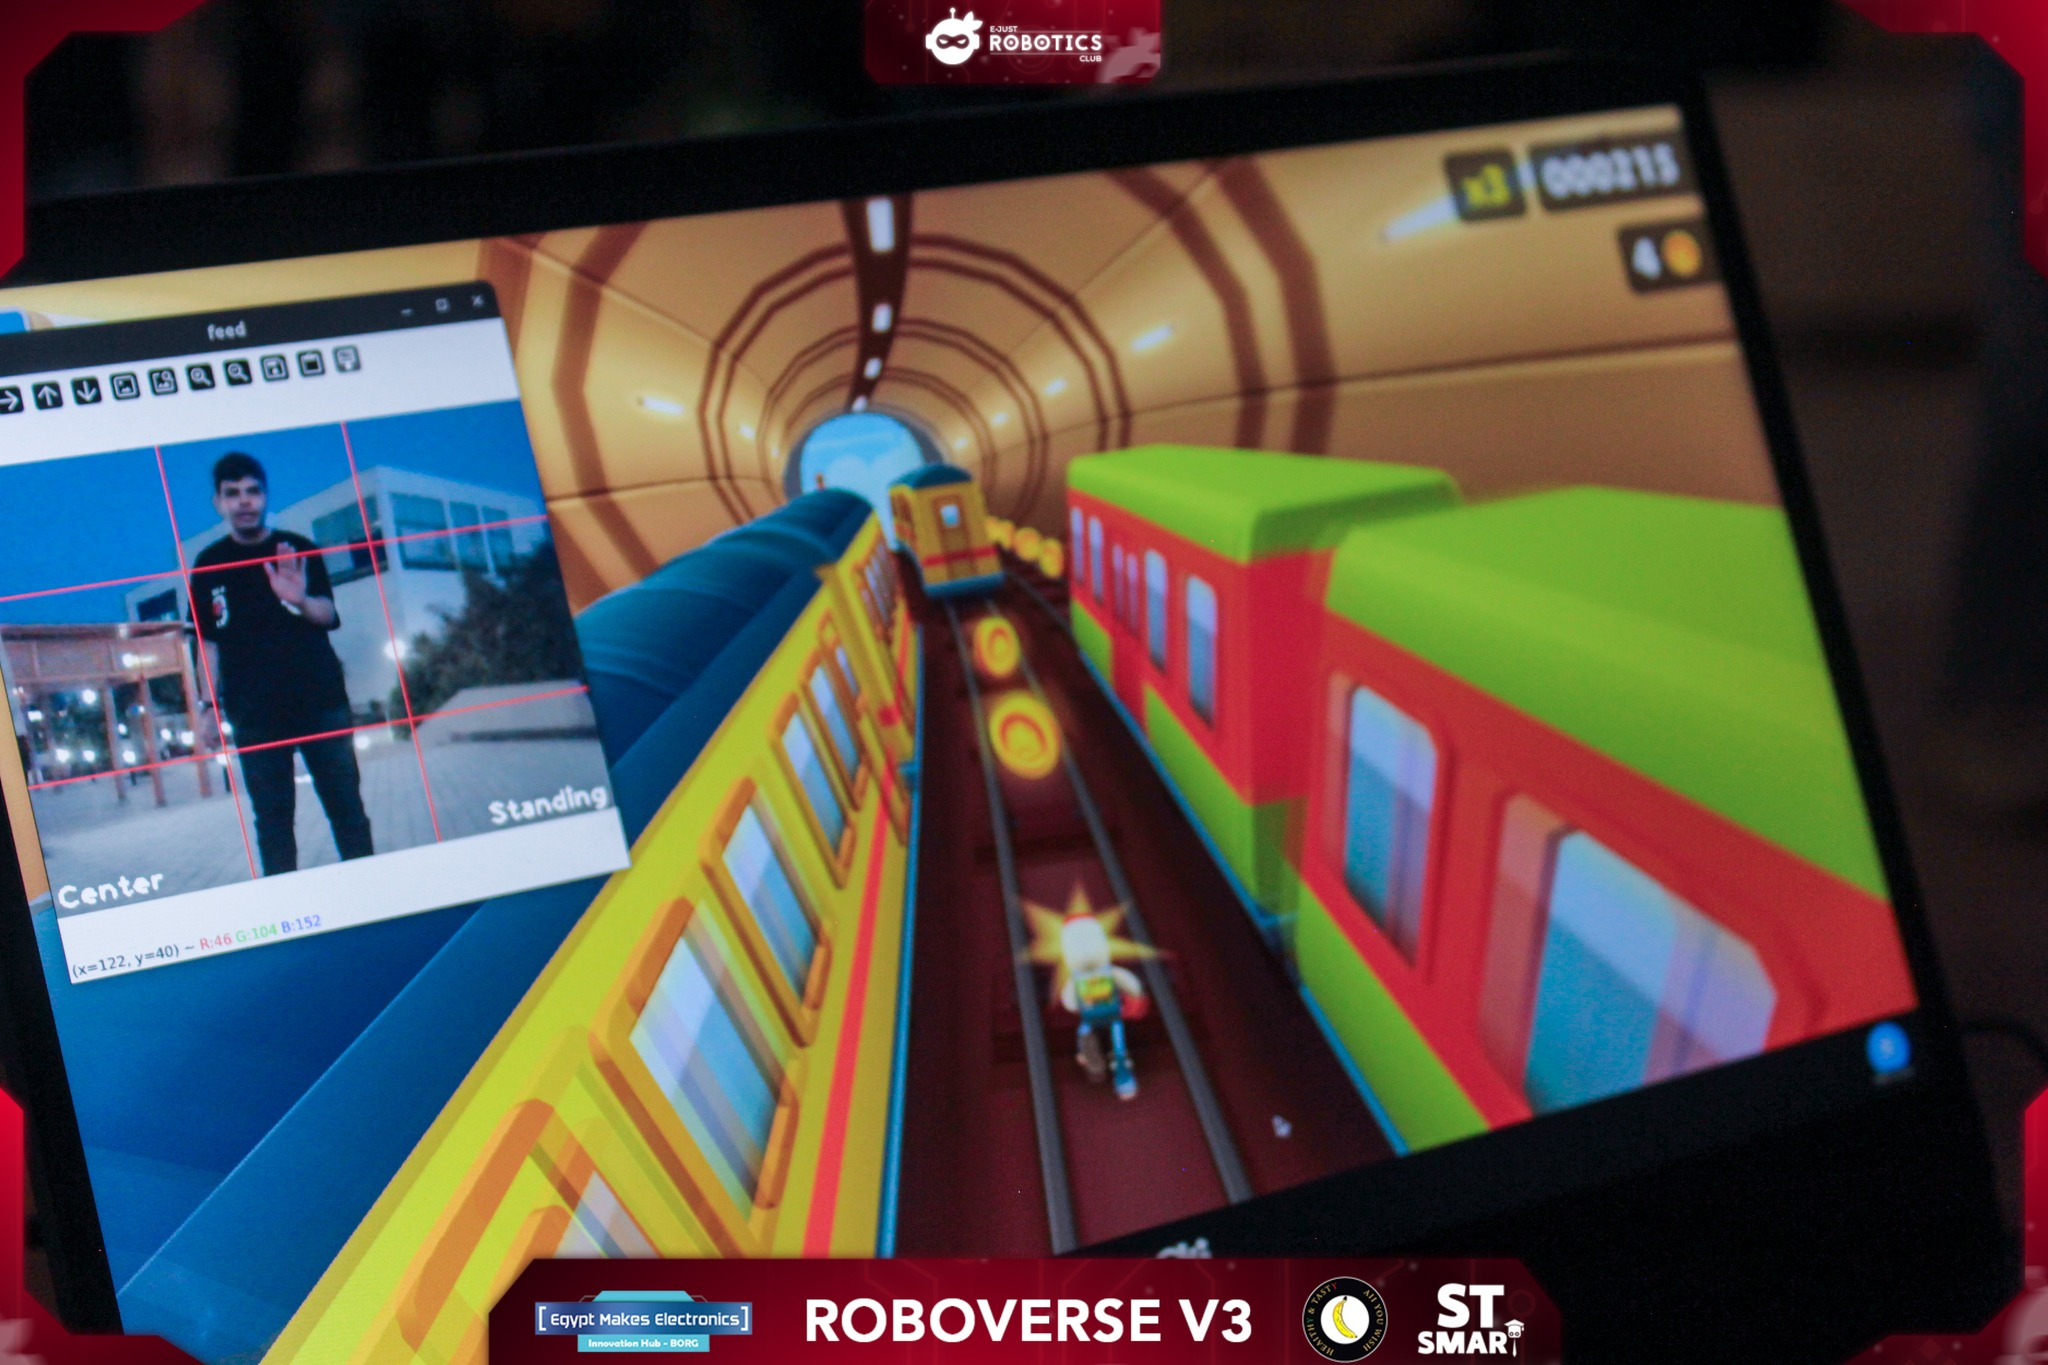
\includegraphics[width=\textwidth]{Images/Entertaining games.jpg}
        
        \label{fig:entertaining1}
    \end{minipage}
    \hfill
    \begin{minipage}{0.48\textwidth}
        \centering
        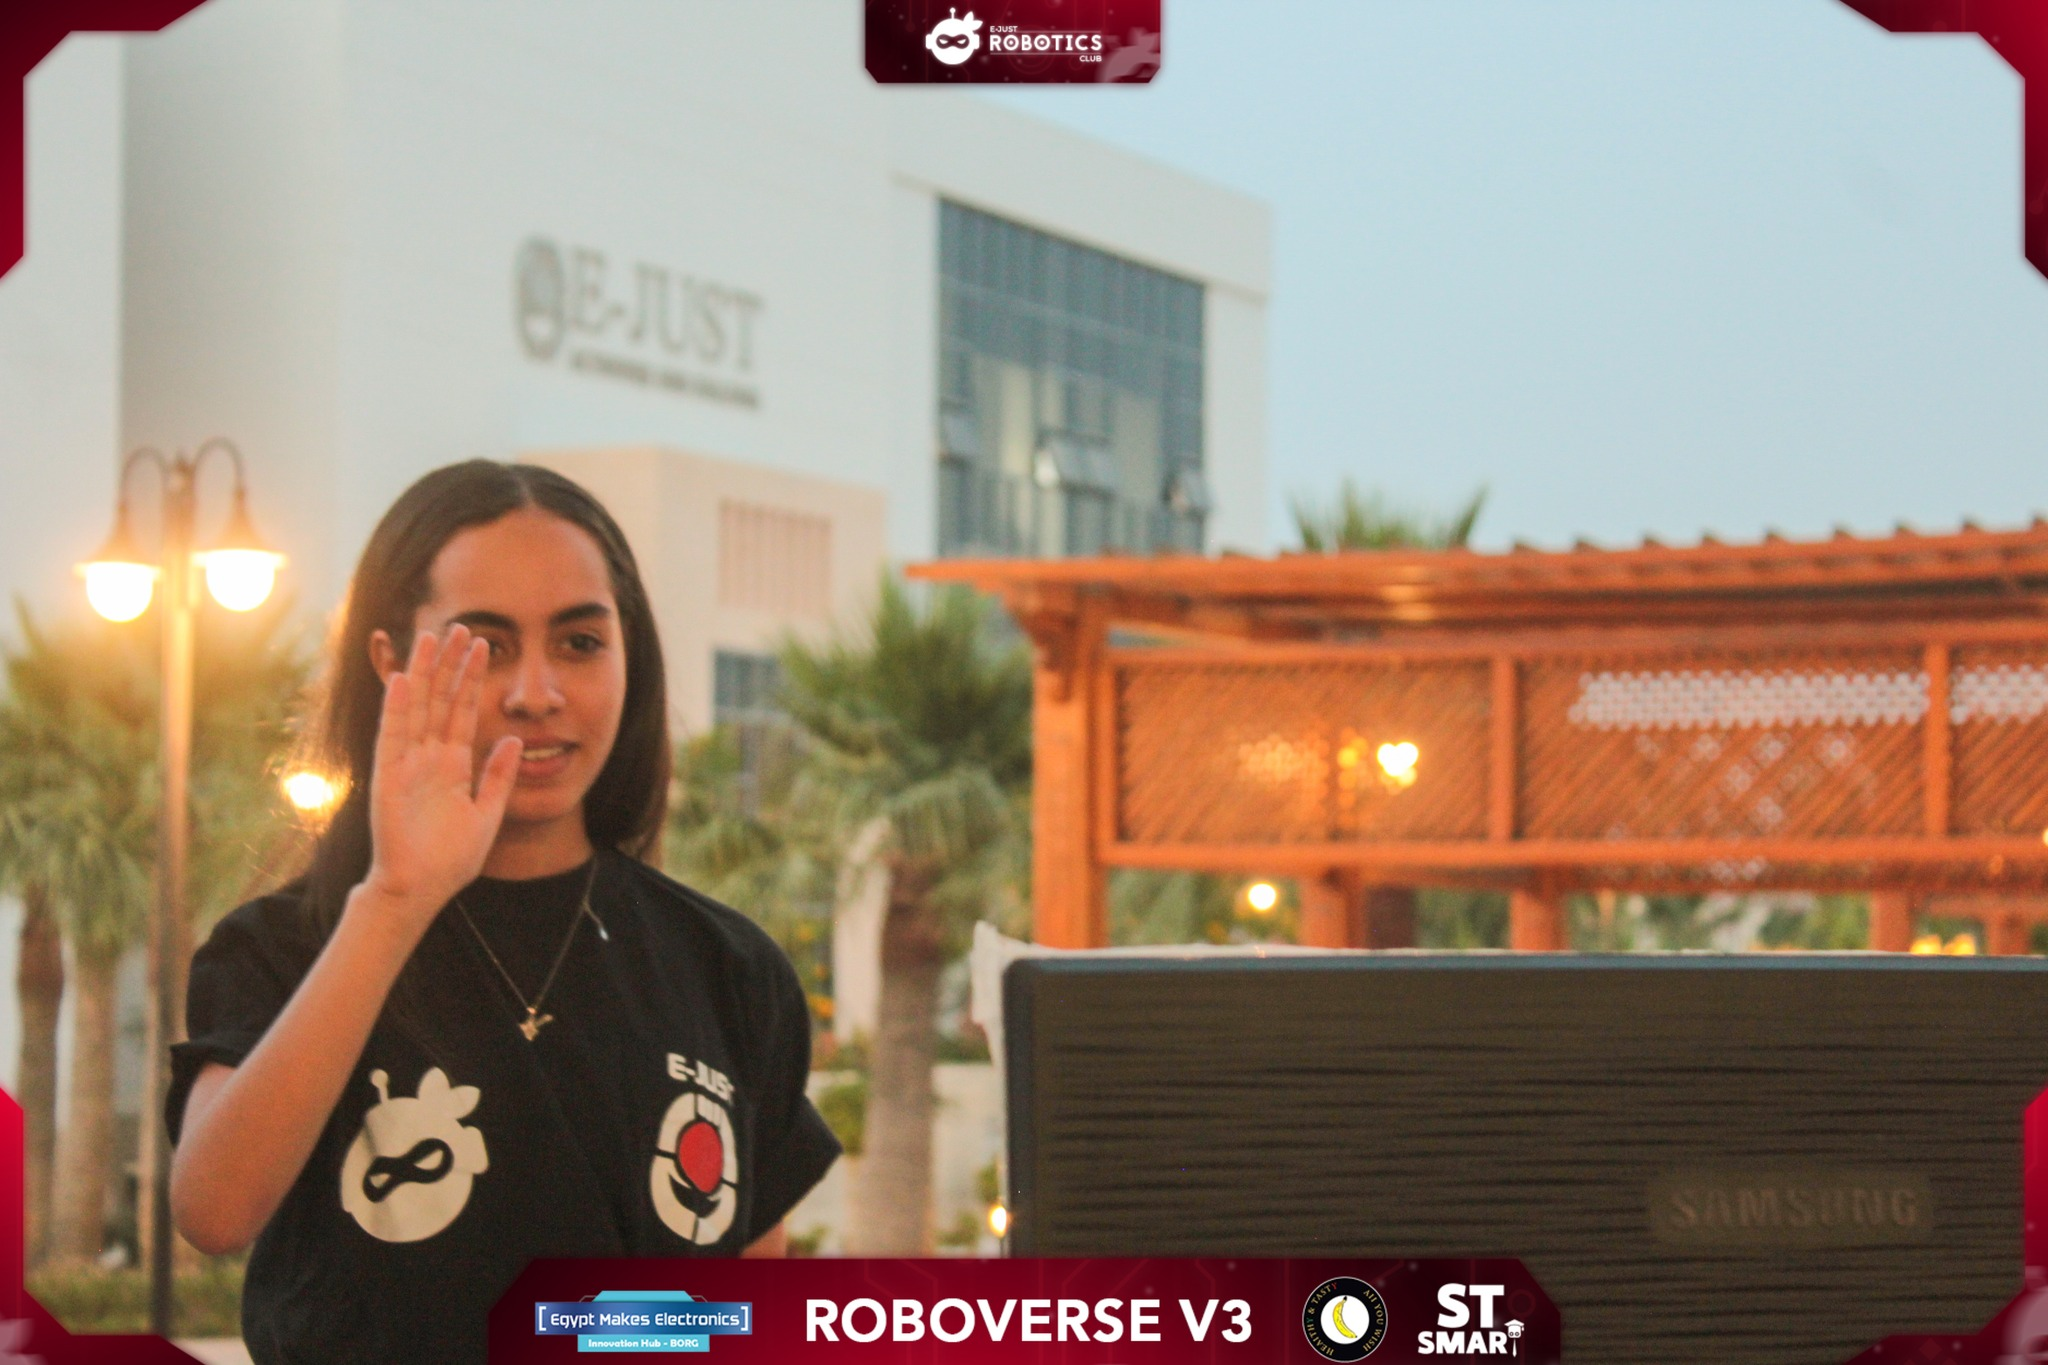
\includegraphics[width=\textwidth]{Images/Entertaining two.jpg}
      
        \label{fig:entertaining2}
    \end{minipage}
    \caption{Games Constructed by our company }
    \label{fig:entertaining}
\end{figure}
\subsubsection{Survey and Event Impact Assessment}
To evaluate the effectiveness of Roboverse 3, a survey was conducted among attendees to assess the knowledge gained and overall experience. The findings were as follows:
\begin{itemize}
    \item Around 77\% of the participants were introduced to new concepts and technologies for the first time.
    \item 21\% of participants expanded their existing knowledge in specific topics.
\end{itemize}
These results underscore the success of the event in promoting education and innovation in robotics and STEM disciplines, reaffirming our club’s commitment to community engagement and technological advancement.

\subsection{Engagement with E-JUST Student Union}
As part of our commitment to foster collaboration within the university, we actively participated in the E-JUST Iftar Day by setting up an interactive booth. This participation allowed us to showcase our club's activities and engage with a broader audience.


\begin{itemize}
    \item Displayed our robotics projects, including the ROV, to introduce attendees to our work and mission.
    \item Provided hands-on experiences, allowing visitors to explore our projects and interact with our technology.
    \item Offered games and interactive challenges to engage students and demonstrate the fun and practical applications of robotics.
\end{itemize}
\begin{figure}[h]
            \centering
            \includegraphics[width=0.75\linewidth]{Images/EJUST Iftar.jpg}
            \caption{Interaction in Iftar day with Prof. Sameh Nada, Vice President of E-JUST}
            \label{fig:iftar}
                \end{figure}

\subsection{ROV for Marine Research and Environmental Sustainability}

Our ROV is designed to contribute to marine research and environmental sustainability by performing a variety of underwater tasks. With its adaptable design, the ROV can integrate various systems to enhance its capabilities and tackle different challenges in marine exploration. 

Key features of our ROV include:
\begin{itemize}
    \item \textbf{High-Resolution Cameras:} Enable detailed underwater exploration, allowing for marine life observation and environmental monitoring.
    \item \textbf{Pneumatic Grippers:} Facilitate object manipulation, supporting tasks such as sample collection and underwater intervention.
    \item \textbf{Collectors:} Designed to gather marine samples for research, aiding in biodiversity studies and pollution assessment.
    \item \textbf{Software Modifications:} Allow real-time adaptability and task-specific programming to meet various operational needs.
    \item \textbf{PCB and Board Customization:} Supports system upgrades, enabling the integration of new technologies for enhanced performance.
\end{itemize}

With its flexible architecture, our ROV can be adapted to perform different tasks that contribute to environmental conservation, from monitoring aquatic ecosystems to assisting in underwater clean-up initiatives. Its modular nature ensures that new technologies and enhancements can be seamlessly incorporated, making it a valuable tool for ongoing marine research and ecological sustainability.



\newpage
\section{Mentoring and Educational Outreach}
Beyond event participation, we prioritize mentoring and knowledge-sharing through workshops and expert-led sessions.

\subsection{Online Seminar on Marine Autonomous Systems}
\textbf{Online Seminar on Marine Autonomous Systems}

\noindent As part of our commitment to knowledge-sharing, we hosted an exclusive online seminar on Marine Autonomous Systems, a field transforming ocean exploration, environmental monitoring, and underwater robotics.
\subsubsection{Attendees}
The seminar was attended by college and high school students who have an interest in submarine robots, especially ROVs.

\subsubsection{Speaker: Eng. Ahmed Abdullah}
\begin{itemize}
    \item \textbf{Club Co-Founder}: Instrumental in establishing E-JUST Robotics Club.
    \item \textbf{Expertise}: Holds a Master’s in Marine Intelligent Robotics from Université de Toulon, France.
    \item \textbf{PhD Candidate}: Norwegian University of Science and Technology in Marine and Maritime Intelligent Robots.

    


\end{itemize}

This seminar provided attendees with in-depth knowledge of marine robotics, the latest technological advancements, and career pathways in this exciting field.

\subsection{Workshops: Bridging the Gap Between Students and Robotics}
To eliminate the gap between students and robotics, we conducted structured workshops addressing different expertise levels. These workshops provided technical knowledge and practical exposure, equipping students with the necessary skills to excel in robotics. Led by 40 mentors and judges, these sessions ensured effective mentorship and hands-on learning opportunities.To ensure the quality of the workshops;after each session, we collected feedback from participants to assess the quality and improve future workshops based on their suggestions.
\begin{figure}[h]
            \centering
            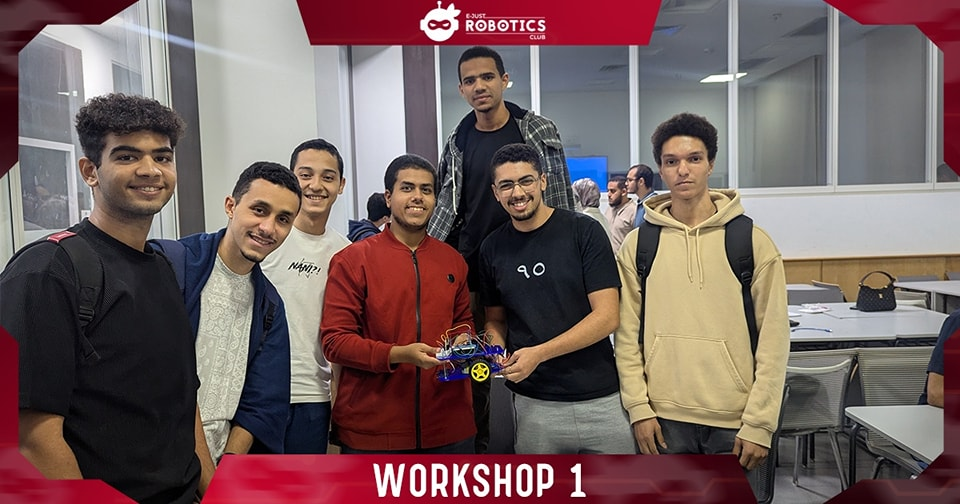
\includegraphics[width=0.7\linewidth]{Images/workshop oo.jpg}
           \caption{Students'engagement in our workshops}
            \label{fig:engagement}
                \end{figure}




\newpage
\subsubsection{Workshop 1: Introduction to Robotics}
Designed for beginners, this workshop provided a foundational introduction to robotics, attracting 70 participants each semester. The sessions covered basic robotics principles, components, and hands-on applications, allowing students to develop an initial understanding and enthusiasm for the field.



\subsubsection{Workshop 2: Advanced Robotics Techniques}
Catering to students who completed Workshop 1 or had prior experience, this workshop focused on advanced concepts, including automation, sensor integration, and algorithm development. With 50 dedicated participants per semester, the workshop fostered deeper technical understanding and encouraged innovative problem-solving in robotics. 

\subsection{Competitions} 

\begin{figure}[h]
    \centering
    \begin{minipage}{0.45\textwidth}
        \centering
        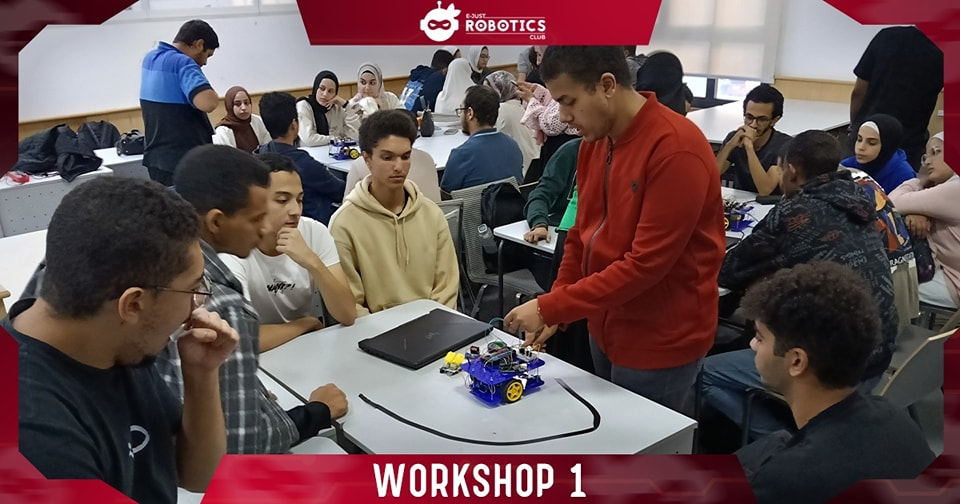
\includegraphics[width=\textwidth]{Images/Workshop1.jpg}
        
        \label{fig:workshop1}
    \end{minipage}
    \hfill
    \begin{minipage}{0.45\textwidth}
        \centering
        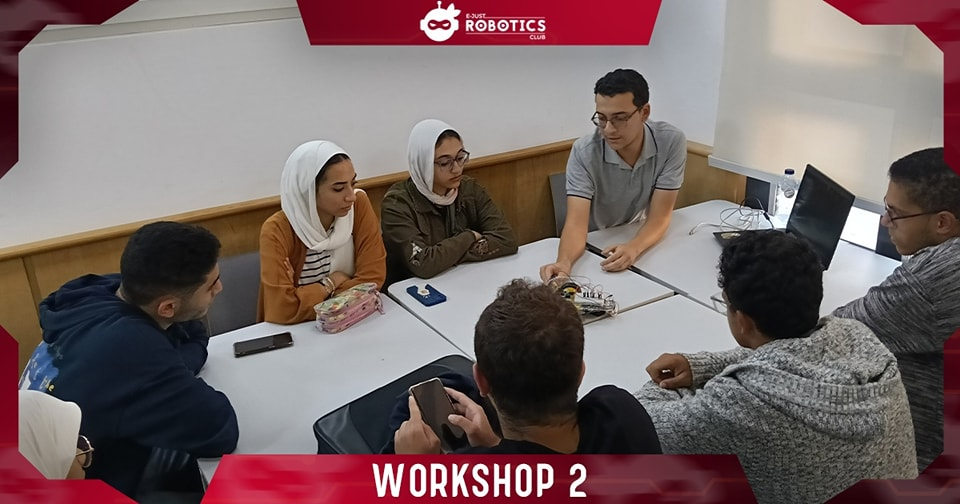
\includegraphics[width=\textwidth]{Images/workshop2.jpg}
      
        \label{fig:worksop2}
    \end{minipage}
    \caption{Our workshops mentoring sessions }
    \label{fig:workshop}
\end{figure}
\subsubsection{Workshop Competitions}
Each workshop series culminates in a hands-on competition, providing participants with an opportunity to apply their acquired skills in real-world scenarios. These competitions foster technical proficiency, problem-solving abilities, and teamwork under pressure. To promote continuous learning, new challenges are introduced in every session. The top three winners are awarded gifts, while all participants receive certificates in recognition of their efforts.
\begin{figure}[h]
            \centering
            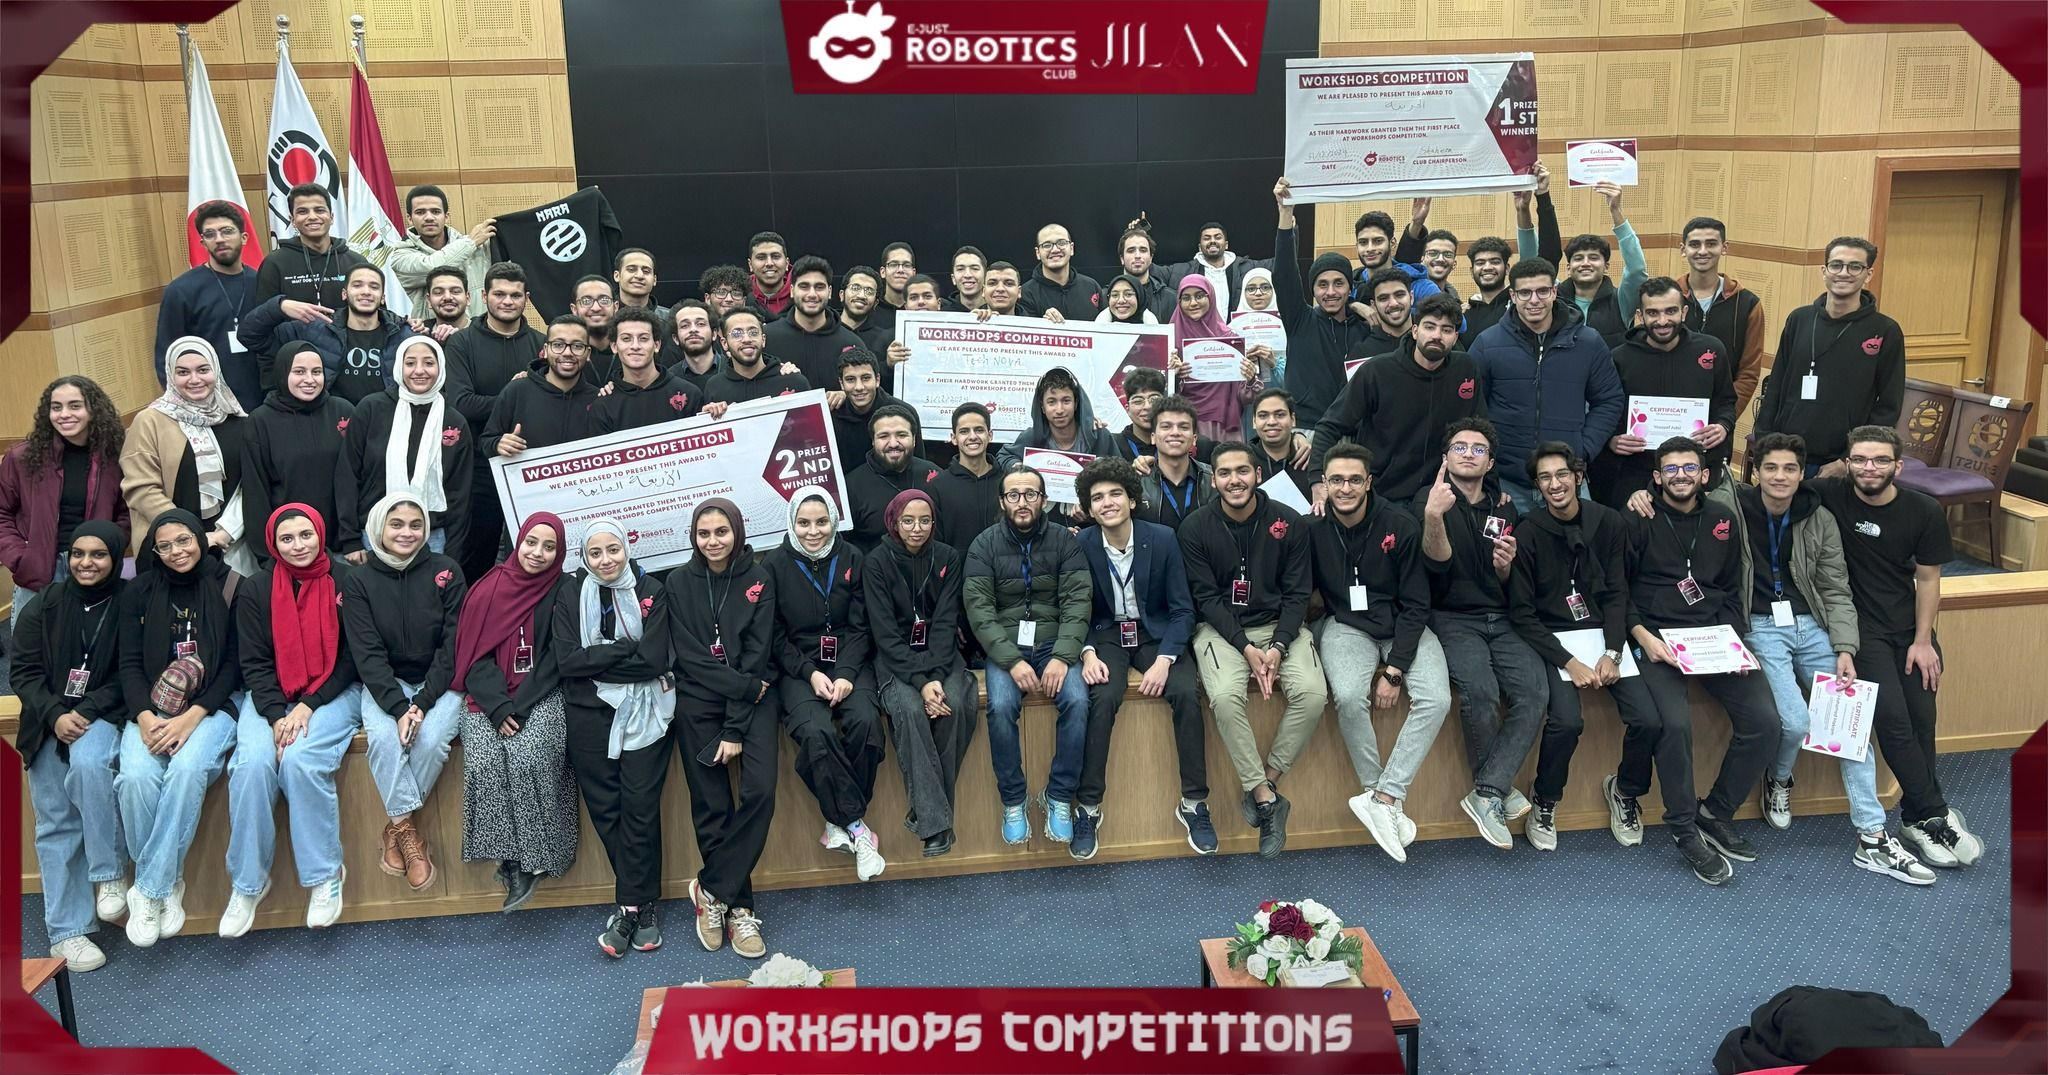
\includegraphics[width=0.65\linewidth]{Images/workshop competition.jpg}
           \caption{All participants in last workshop competitions}
            \label{fig:enter-label}
                \end{figure}







\newpage
\subsection{Robot Programming Rally (RPR)}
As part of our commitment to fostering young talent in robotics, we partnered with EME Innovation Hub - BORG and Jupiter Academy to organize the Robot Programming Rally (RPR). Our technical team played a crucial role as mentors, offering guidance, technical support, and expertise to young participants throughout the competition. By engaging in this initiative, we helped nurture problem-solving skills, teamwork, and hands-on robotics experience for aspiring engineers, emphasizing the integration of STEM principles in robotics education.

\subsection{MEKATRO Sessions}
We host MEKATRO sessions for students at E-JUST. These sessions cover various topics in robotics and are conducted by professors and engineers specializing in different areas such as Reinforcement Learning, ROS (Robot Operating System), LaTeX, and more. Each session is meticulously planned to provide students with valuable insights and practical knowledge from experts in the field.

To ensure widespread access to these sessions, we utilize social media platforms to broadcast them either through recorded videos or live streams on our channels. This approach enables everyone, regardless of location, to benefit from the valuable information shared during these sessions.

Our two latest sessions included:
\begin{itemize}
    \item \textbf{February 29, 2024}: Attended by over 180 students.
    \item \textbf{March 5, 2024 – Machine Learning Session by Eng. Abdullah Elameer}: This session, attended by 125+ participants, provided an in-depth explanation of machine learning models, including supervised, unsupervised, and reinforcement learning techniques.
\end{itemize}

\begin{figure}[h]
    \centering
    \begin{minipage}{0.48\textwidth}
        \centering
        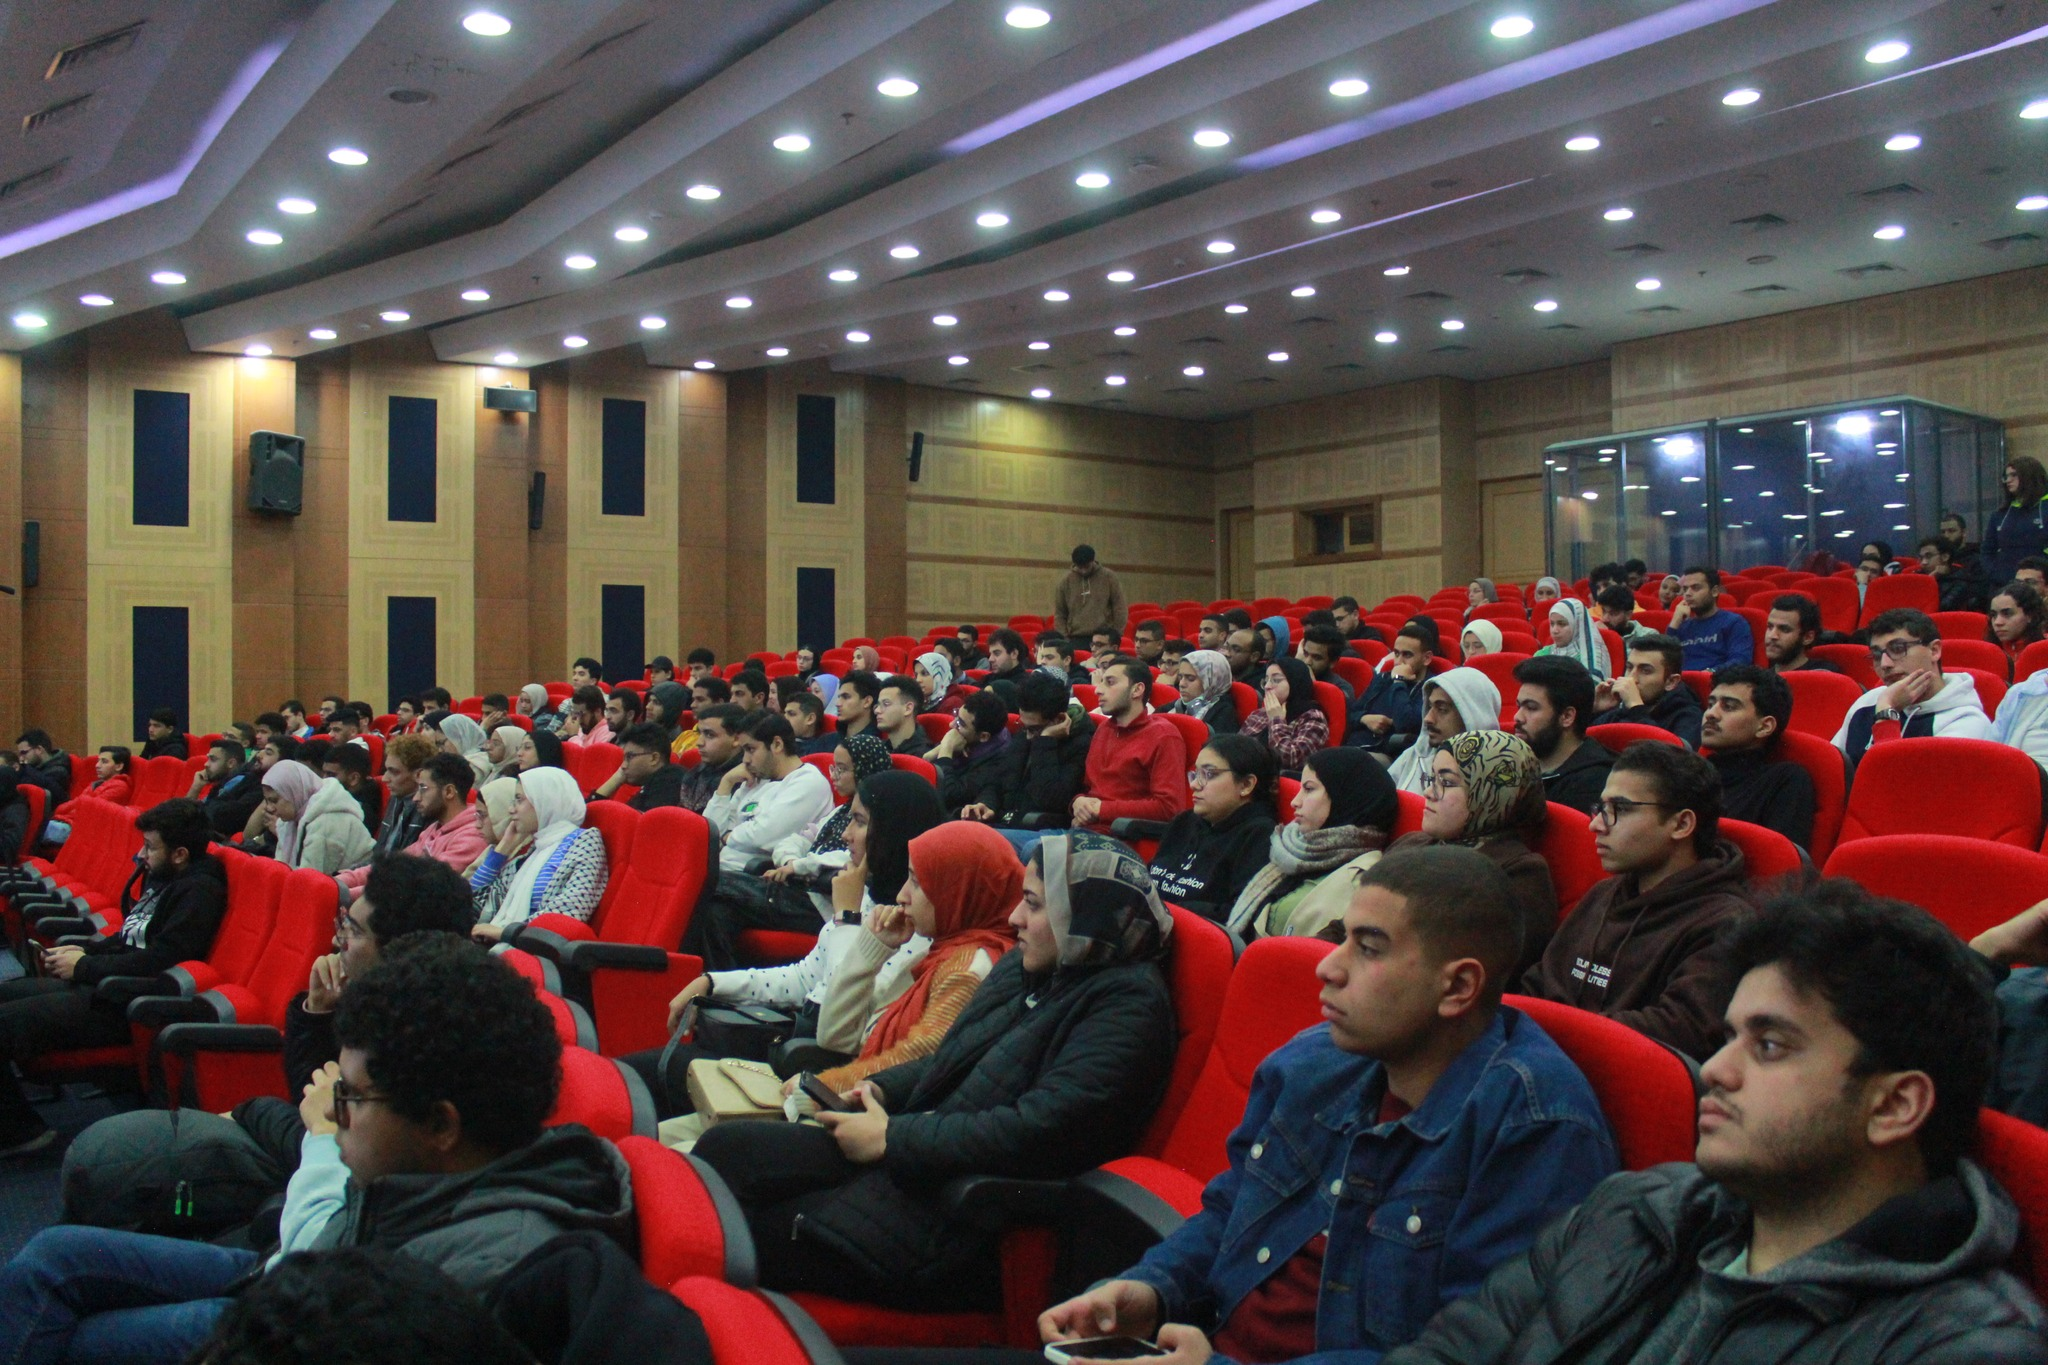
\includegraphics[width=\textwidth]{Images/Mekatro1.jpg}
        
        \label{fig:mekatro1}
    \end{minipage}
    \hfill
    \begin{minipage}{0.465\textwidth}
        \centering
        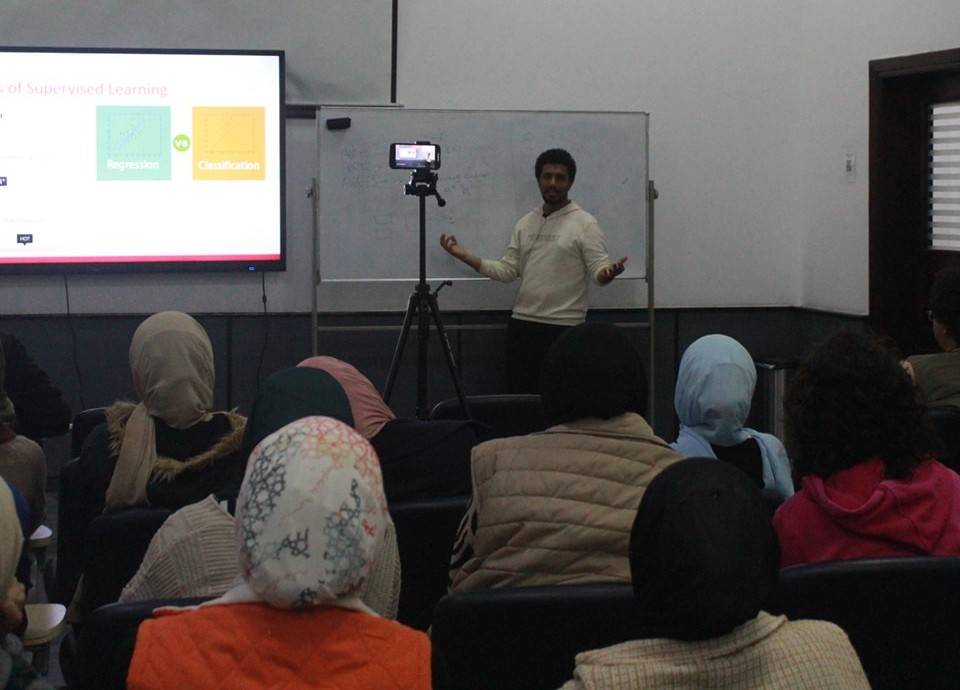
\includegraphics[width=\textwidth]{Images/ameer's session .jpg}
      
        \label{fig:mekatro2}
    \end{minipage}
    \caption{Pictures from MEKATRO Sessions}
    \label{fig:mekatro}
\end{figure}

\newpage
\section{Media Outreach}
We expanded our media outreach in 2023 and 2024 by establishing four media contacts and distributing press releases across four outlets to showcase our robotics education and community initiatives. These collaborations helped us engage a diverse audience, including students, educators, and community members, inspiring greater participation in our programs, workshops, and events while fostering awareness about the impact of robotics in education and innovation.

\subsection{Media Contacts}
We collaborated with:
\begin{itemize}
    \item \href{https://www.facebook.com/E-JUST.official/videos/3449961901956390/}{Al Yom HD}
    \item \href{https://www.facebook.com/Channel1/videos/555933573138009/}{Channel 1}
    \item \href{https://www.facebook.com/ElWatanNews/videos/176552042188662}{El-Watan News}
    \item \href{https://www.facebook.com/watch/?mibextid=6p5qLk&v=1074663143567405}{CTV}
    
\end{itemize}

\subsection{Press Releases}
The dissemination of press releases in various outlets helped us extend our reach and attract new participants to our workshops, competitions, and educational sessions, contributing to the growth and sustainability of our robotics club.
Our press releases appeared in:
\begin{itemize}
    \item \href{https://rb.gy/maf8ra}{Ahram Masr}
    \item \href{https://daralmaref.com/News/1604649.aspx}{Dar Al-Maref}
    \item \href{https://rb.gy/n0l5f6}{Akhbar El-Yom}
    \item\href{https://www.elwatannews.com/news/details/7423221#goog_rewarded}{Masrawy}
    \item\href{https://www.elwatannews.com/news/details/7423221#goog_rewarded}{El-Watan News}
\end{itemize}
\begin{figure}[h]
    \centering
    \begin{minipage}{0.46\textwidth}
        \centering
        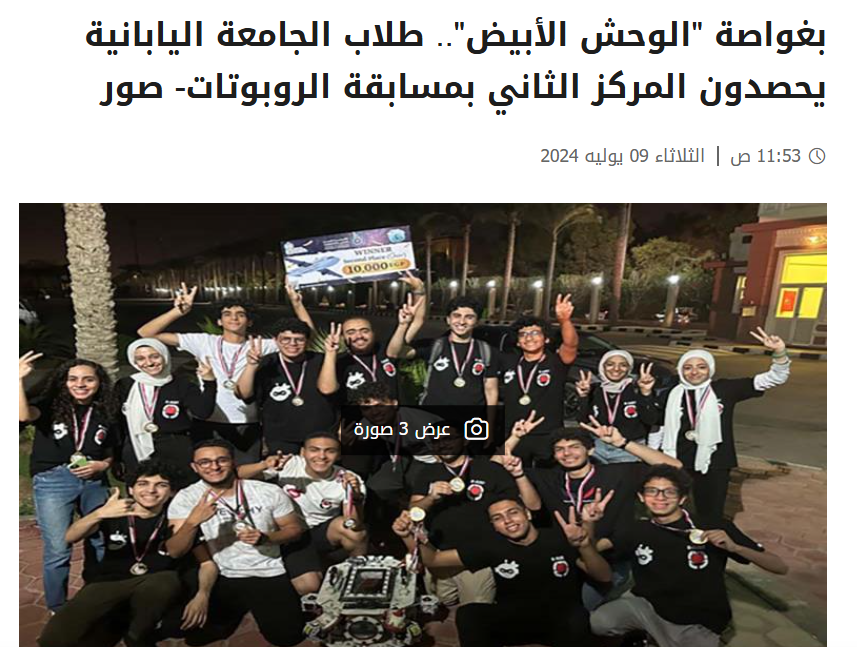
\includegraphics[width=\textwidth]{Images/Masrawy.png}
        
        \label{fig:masrawy}
    \end{minipage}
    \hfill
    \begin{minipage}{0.44\textwidth}
        \centering
        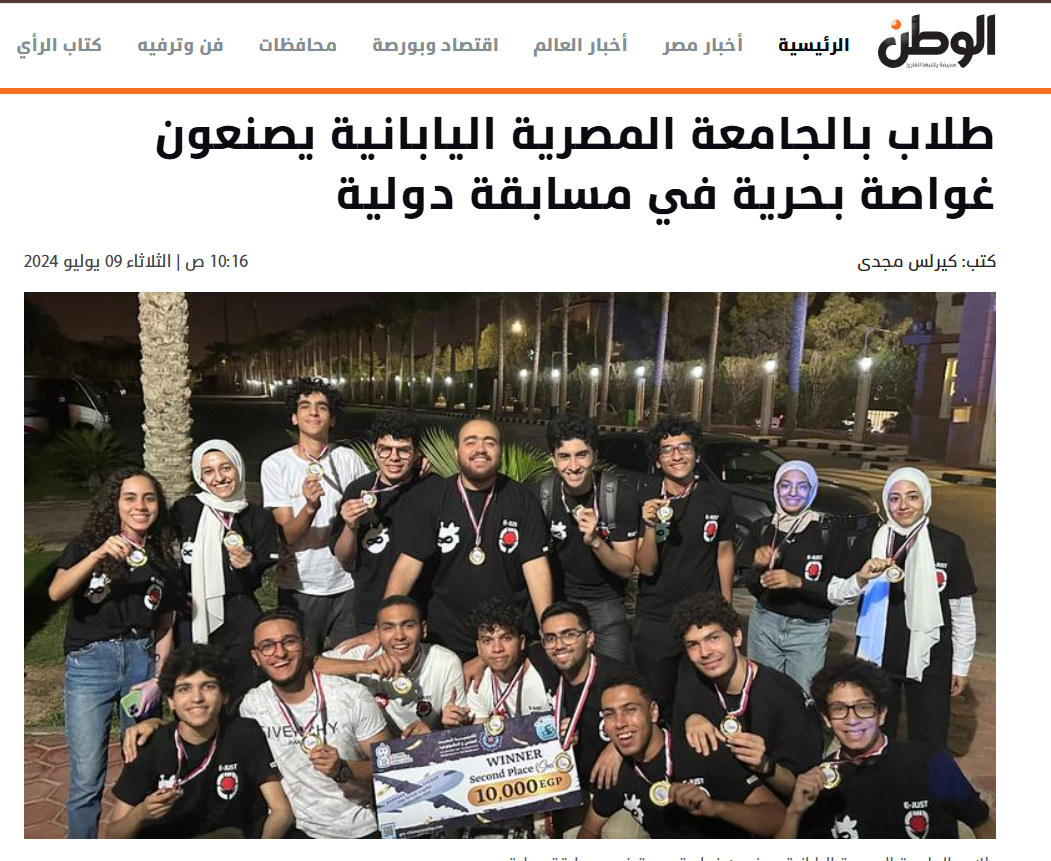
\includegraphics[width=\textwidth]{Images/Elwatan news.png}
      
        \label{fig:elwatan}
    \end{minipage}
    \caption{Media Cover for our achievements }
    \label{fig:news}
\end{figure}


\end{document}
